% Preamble
\documentclass[12pt, a4paper, twoside]{article}
\usepackage[a4paper, left=0.75in, right=0.75in, top=1in, bottom=1in]{geometry}
\usepackage{lipsum, verbatim, fancyhdr, lastpage, graphicx, hyperref, amsmath} % indentfirst 
\usepackage[backend=bibtex]{biblatex}
\graphicspath{{./plots/}}
\addbibresource{ref.bib}
% Top Matter
\hypersetup{
	colorlinks   = true,
	urlcolor     = blue, 
	linkcolor    = blue, 
	citecolor   = red
}
\pagestyle{fancy}
\fancyhead[CO, CE]{CS 725: Foundations of Machine Learning (Autumn 2023) --- Project}
\fancyhead[LO, LE, RO, RE]{}
\fancyfoot[CO, CE]{Page \thepage\ of \pageref{LastPage}}
\fancyfoot[LO, LE, RO, RE]{}
% \bibliographystyle{plain}

\title{\vspace{-0.5in}\textbf{CS 725: Foundations of Machine Learning \\
		Calorie Estimation of Food item from Images}}
\author{CV Mavericks\footnote{The project has undergone revisions based on the feedback provided on 18/10/2023. Initially, the project focused on \emph{Image-Based Disease Diagnosis using Deep Learning}. The new project concept has received approval from Krishnakant Bhatt (21q050016@iitb.ac.in).}\\
	23m2154, 23m2156, 23m2157, 23m2158, 23m2162}
\date{November 28, 2023}

% Main Matter
\begin{document}
	\maketitle
	\thispagestyle{fancy}
	
	\begin{abstract}
		Our project addresses the limitations of current food image datasets in accurately estimating calories. We introduce a food image dataset that includes both food annotations and detailed volume and mass records for each item, along with a calibration reference. Our dataset comprises 2978 images, each accompanied by annotations and essential food metrics. To estimate the calorie content of food in this dataset, we employ a deep learning approach utilizing YOLO for food detection and a GrabCut algorithm to outline the contours of each food item. With this information, we calculate the volume and subsequently, the calorie content of each food.
	\end{abstract}
	
	\section{Problem Statement}
	Estimating the calorie content from food images requires the food image datasets which faces a critical challenge in accurately estimating calorie content due to the choice of object detection algorithm and volume estimation method. This project aims to fill this gap by using a detailed food image dataset provided by ECUST\cite{liang}. It includes precise food annotations, along with volume, mass records, and a reliable calibration reference (one Yuan coin) for each item. This dataset is a collection of 2978 images, each meticulously annotated and supplemented with necessary food metrics i.e. volume, density, calorie content etc. To achieve accurate calorie estimation, a deep learning methodology is employed. This involves the adaptation of You Only Look Once (YOLO) for precise food detection, followed by the implementation of the GrabCut algorithm to precisely outline the contours of each food item. The segmented images would be utilized to calculate the volume and, subsequently, the calorie content of each food item.
	\par
	The project aims to address two key challenges in dietary assessment from food images:
	\begin{description}
		\item[Detection and Classification of Food Items:] Accurate identification and categorization of food items from images represent the initial hurdle. Existing methodologies often fall short in providing precise detection and classification. This project seeks to leverage advanced techniques, particularly YOLO, to enhance the capability to not only detect but also classify food items within images. By employing YOLO, the system aims to achieve an improvement in the accuracy and efficiency of food item recognition.
		
		\item[Estimation of Food Volume for Calorie Content Determination:] 
		The second significant challenge lies in estimating the volume of identified food items, a crucial step in determining their calorie content. Traditional approaches struggle to provide the necessary precision for this task. To overcome this limitation, the project proposes the integration of GrabCut, an advanced segmentation algorithm. By applying GrabCut, the system aims to accurately delineate the contours of each food item, enabling precise volume estimation. This, in turn, facilitates a more accurate and reliable assessment of calorie content.
	\end{description}
	\par
	By combining YOLO for food item detection and classification with GrabCut for precise volume estimation, this project seeks to accurately estimate the calorie content from food images. The successful execution of this approach promises to benefit individuals seeking improved dietary choices, weight management, fitness goals, and specific dietary requirements.
	
	\section{Proposed Solution Approach}
	The solution methodology for estimating the calorie content from food images can be summarized as follows:
	\begin{description}
		\item[Object Detection:] Our aim is to help people who want to keep track of the calories they consume. We would create a system that works with a smartphone. Before eating, users need to take pictures of their food from the top and side views. They should include a One Yuan coin in each picture. For the top view, we use YOLO to recognize the types of food and draw an outline or bounding box around them in the photos. We do the same for the side view. We reframe object detection as a single regression problem, straight from image pixels to bounding box coordinates and class probabilities. Using our system, you only
		look once (YOLO) at an image to predict what objects are
		present and where they are. YOLO is refreshingly simple. A single convolutional network simultaneously predicts multiple bounding boxes and class probabilities for those boxes. YOLO trains on full images and directly optimizes detection performance. This unified model has several benefits over traditional methods of object detection.
		
		\item[Image Segmentation:] Before figuring out the volume, we first break down each box into its separate parts. We would use something called GrabCut algorithm. It's a way to process images that helps us focus on specific areas. Normally, users would have to highlight areas themselves, but we've made it so the system can do this on its own. After this step, we get a precise outline or contour of each food item. Then, we can estimate the volume and calorie content. This process uses an image processing approach to segment each bounding box. As mentioned above, the bounding boxes around the object that GrabCut needs can be provided by YOLO. After segmentation, we can get a series of food images stored in matrix, but with the the values of the background pixels being replaced by zeros. This will leave only the foreground pixels.
		
		\item[Calorie Estimation:] The user needs to provide the image clicked from both side and top view along with the One Yuan coin. According to the One Yuan coin detected in the top view, the true size of a pixel is known. Similarly, we know actual size of of a pixel in the side view. Then we use different formulas to estimate volume of each food. After getting volume, food’s calorie is obtained by searching related calorie tables. 
	\end{description}
	
	
	\section{Datasets}
	We utilize the ECUST dataset, which encompasses 19 diverse food types including apple, banana, bread, bun, doughnut, egg, fired doughnut, grape, lemon, litchi, mango, mooncake, orange, peach, pear, plum, kiwi, sachima, and tomato as shown in Figure \ref{F:table}. The model is trained on a total of 2978 images from this dataset. Each food item is captured in multiple sets of photos, showcasing both its top and side views (see Figure \ref{F:sample}). Each image is calibrated using a one Yuan coin as shown in Figure \ref{F:coin}, and no more than two food items are present in a single picture. Additionally, all images in the dataset are smaller than 1000 by 1000 pixels. The dataset provides density and energy content information for all 19 food items.
	\par
	To ensure accurate measurement of food volume and mass, foods that are sufficiently large, stable, and less likely to deform. are selected. Foods with small volumes, like peanuts, are challenging to measure accurately and can lead to significant errors when compared to their actual volume. In ECUST dataset, every food item is presented in its entirety. In the dataset, the whole foods, such as entire apples rather than sliced ones were prioritized to facilitate volume and weight measurements. Photos were taken in various mobile devices, under lighting conditions, including low light settings. Different shooting angles were used for top and side views. The position of the food in images was flexible, as long as it was fully captured. A One Yuan coin was chosen as the calibration object due to its common availability, with a diameter of 25.0mm.
	
	\begin{figure}[p]
		\centering
		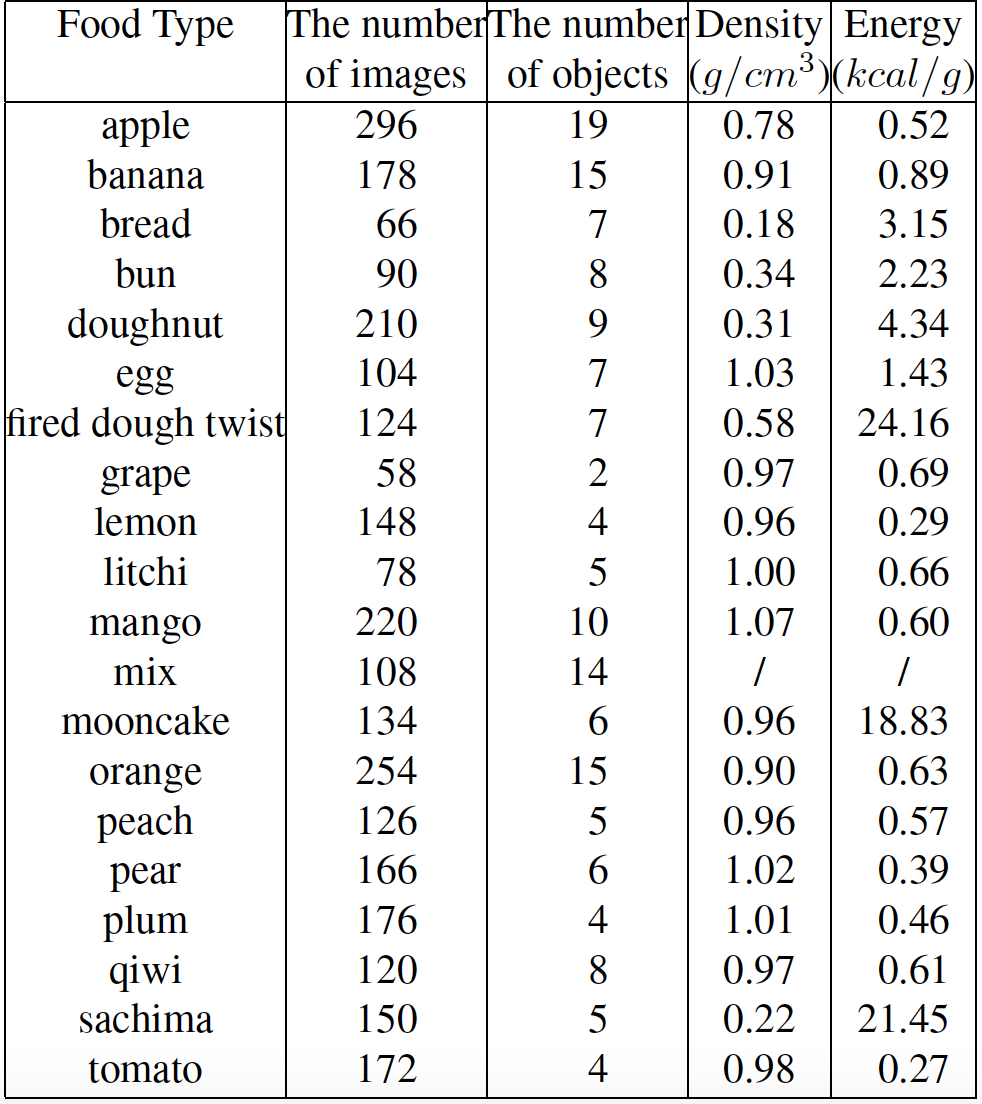
\includegraphics[width=\textwidth]{table}
		\caption{Details of food item from ECUST dataset}
		\label{F:table}
	\end{figure}
	\begin{figure}[p]
		\centering
		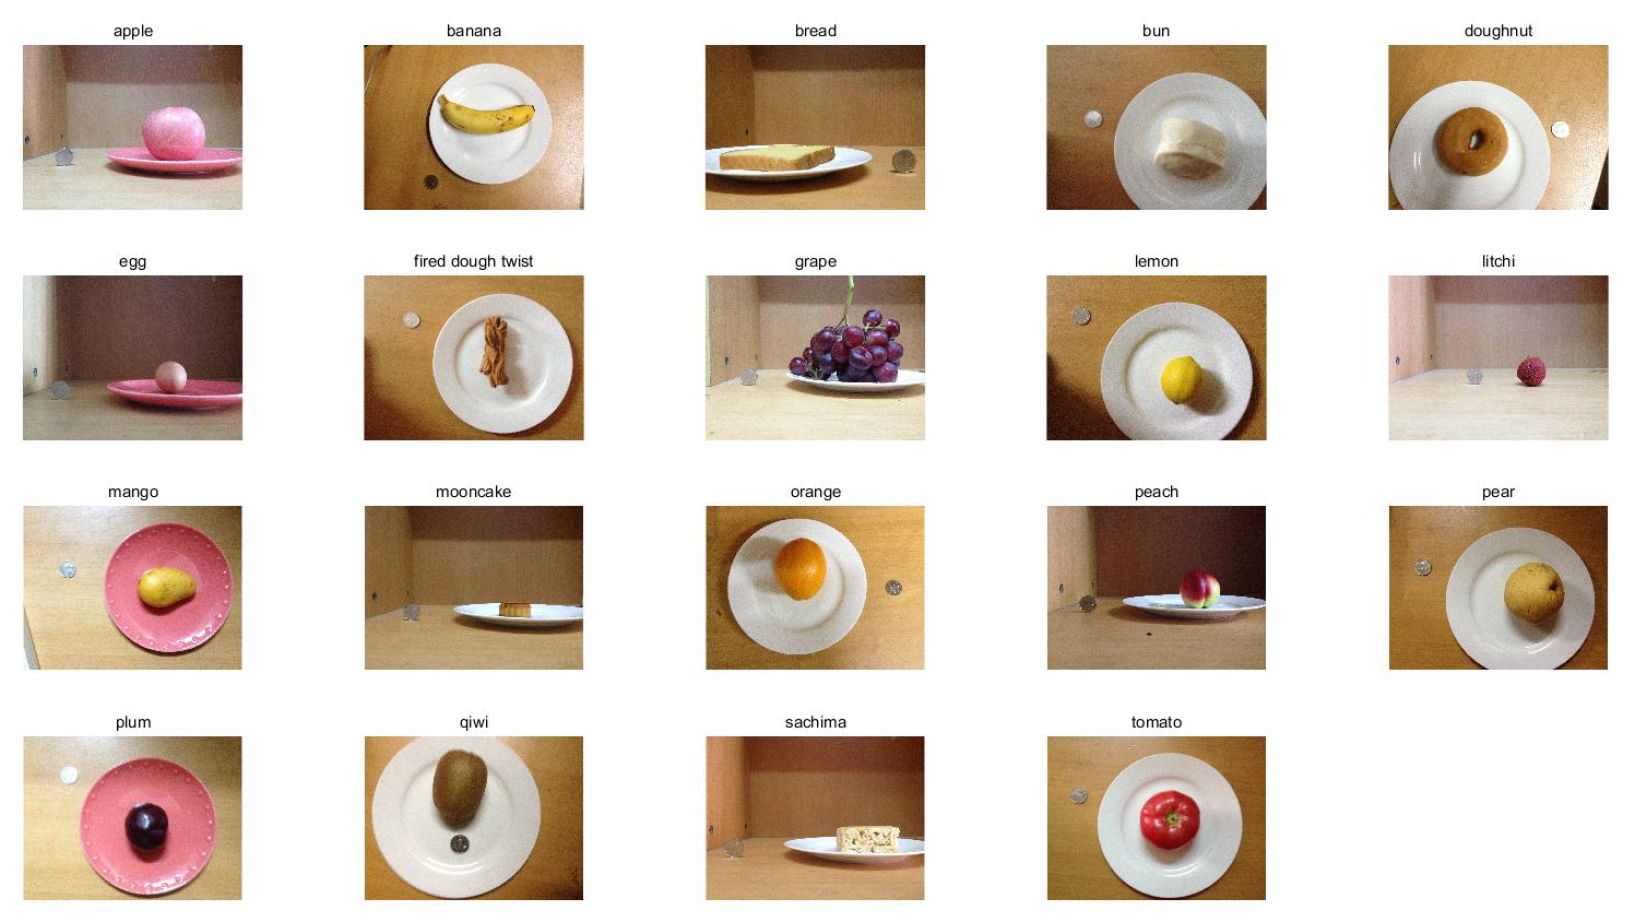
\includegraphics[width=\textwidth]{sample}
		\caption{Sample food items from ECUST dataset}
		\label{F:sample}
	\end{figure}
	\begin{figure}[p]
		\centering
		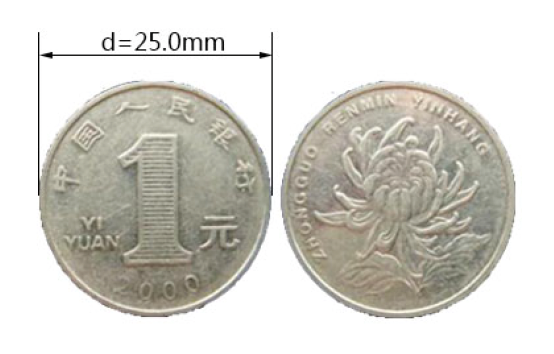
\includegraphics[width=0.75\textwidth]{coin}
		\caption{Dimension of One Yuan coin}
		\label{F:coin}
	\end{figure}
	
	\section{Implementation Details}
	\subsection{YOLO}
	This algorithm\cite{yolo} takes an image as input and produces a convolution feature map. We unify the separate components of object detection into a single neural network. Our network uses features from the entire image to predict each bounding box. It also predicts all bounding boxes across all classes for an image simultaneously. This means our network reasons globally about the full image and all the objects in the image. The YOLO design enables end-to-end training and realtime speeds while maintaining high average precision. Our system divides the input image into an S × S grid. If the center of an object falls into a grid cell, that grid cell
	is responsible for detecting that object. Each grid cell predicts B bounding boxes and confidence scores for those boxes. These confidence scores reflect how
	confident the model is that the box contains an object and also how accurate it thinks the box is that it predicts. Formally we define confidence as $Pr(Object) \times IOU^{truth}_{pred}$ . If no object exists in that cell, the confidence scores should be
	zero. Otherwise we want the confidence score to equal the intersection over union (IOU) between the predicted box and the ground truth.
	Each bounding box consists of 5 predictions: x, y, w, h, and confidence. The (x, y) coordinates represent the center of the box relative to the bounds of the grid cell. The width and height are predicted relative to the whole image. Finally the confidence prediction represents the IOU between the predicted box and any ground truth box.
	Each grid cell also predicts C conditional class probabilities, $Pr(Class_i
	|Object)$. These probabilities are conditioned on the grid cell containing an object. We only predict one set of class probabilities per grid cell, regardless of the
	number of boxes B. At test time we multiply the conditional class probabilities and the individual box confidence predictions,
	\begin{equation}
		Pr(Class_i|Object) \times Pr(Object) \times IOU^{truth}_{pred} = Pr(Class_i) \times IOU^{truth}_{pred}
	\end{equation}

	which gives us class-specific confidence scores for each box. These scores encode both the probability of that class appearing in the box and how well the predicted box fits the object.
	For evaluating YOLO on PASCAL VOC, we use S = 7, B = 2. PASCAL VOC has 20 labelled classes so C = 20.
	Our final prediction is a 7 × 7 × 30 tensor
	
	\subsection{GrabCut Algorithm}
	The GrabCut algorithm\cite{grabcut} employs Image Segmentation. In this method, we use a box to define the object, effectively separating it from the background. The outer region of the box represents the background, while the inner portion combines some background and the object. Subsequently, an iterative process designates each pixel as either background or foreground. Initially, the computer makes an educated guess based on user-provided data. Then, we utilize a Gaussian mixture model to characterize both the foreground and background. Next, we label pixels as probable foreground or probable background, designating others as unknown.
	\par
	In this algorithm, every pixel becomes a node in a graph. Additional nodes like source and sink nodes are introduced. The source node connects to the foreground pixels, while the sink node connects to the background pixels. The likelihood of a pixel being foreground or background influences the edge weights connecting the pixels to these nodes. The similarity between pixels, indicated by the edge information, determines these weights. If there's a substantial color difference between pixels, a low weight is assigned to the edge. Following this, the graph undergoes Segmentation using min-cut. This operation divides the graph into two parts, separating the source and sink nodes, and does so with the least possible cost. The total weights of the cut edges constitute the cost function. Post-cut, all pixels connected to the Source node become foreground, while those linked to the Sink node become background. This process continues until the classification stabilizes.
	
	\subsection{Volume Calculation}
	To estimate the volume\cite{vol}, we calculate the scale factors based on calibration objects. We use a One Yuan coin to show the specific process of calculating the volume. The diameter of the coin is 2.5 cm, and the side view’s and top view's scale factor ($\alpha_S$ and $\alpha_T$) is calculated with Equation \ref{E:as} and \ref{E:at}.
	\begin{align}
		\alpha_S &= \frac{2.5}{(W_S + H_S)/2} \label{E:as}\\
		\alpha_T &= \frac{2.5}{(W_T + H_T)/2 \label{E:at}}
	\end{align}
	\par
	Where $W_S$ and $H_S$ are the width and height of bounding box in side view. Moreover, $W_T$ and $H_T$ are the width and height of bounding box in top view.
	\par
	Furthermore, we divide the foods into three categories based on shape: ellipsoid, column, irregular. Different volume estimation formula will be selected for different types of food, according to Equation \ref{E:vol}. 
	\begin{equation}\label{E:vol}
		v = 
		\begin{cases}
			\beta \cdot \frac{\pi}{4} \cdot \alpha_S^3 \cdot \sum_{k=1}^{H_S} (L^k_S)^2, &\text{if shape is ellipsoid} \\
			\beta \cdot  s_T \cdot \alpha_T^2 \cdot H_S \cdot \alpha_S, &\text{if shape is column} \\
			\beta \cdot  s_T \cdot \alpha_T^2 \cdot \alpha_S \cdot \sum_{k=1}^{H_S} \left(\frac{L^k_S}{L_S^{max}}\right)^2, &\text{if shape is irregular} 
		\end{cases}
	\end{equation}
	\par
	Where $L^k_S$ is the number of foreground pixels in side view of row $k$ ($k \in 1, 2, 3, \dots , H_S$). $L^{max}_S = \max_{k} L^k$, it records the maximum number of foreground pixels in side view. $\beta$ is a compensation factor (default value = 1.0).  $s_T$ is the surface area of the top view.
	\par
	After estimating the volume, the next step is to estimate each food’s mass ($m$ in $g$). It can be calculated in Equation \ref{E:mass}, Where $v$ represents the volume of food in $cm^3$, and  $\rho$ represents its density value in $g/cm^3$. Then the calorie ($C$ in $cal$) of the food can be calculated by Equation \ref{E:cal} using the unit energy ($c$ in $cal/g$).
	\begin{align}
		m &= \rho \cdot v \label{E:mass} \\
		C &= c \cdot m \label{E:cal}
	\end{align}
	\par
	The density, unit energy values and shape for each food items can be obtained from ECUST dataset.
	
	\section{Results}
	The main results are as follows:
		\begin{itemize}
		\item Volume estimation results are shown in the below figure. For most types of food in our experiment, the estimation volume are closer to reference volume.
		\item We use mean error as the evaluation metric for the volume estimation of each of the food item class. It is assumed that within a single food class, the estimated volume is either overestimated or underestimated for all the instances.
		\begin{equation}
			ME = \sum_{k=1}^{N} \frac{v_{true}^k-v_{pred}^k}{v_{true}^k}\times 100 \%
		\end{equation}
		\item The mean error between estimation volume and true volume does not exceed 20\% except banana, grape, bread. For some food types such as lemon, orange, tomato, our estimation result is close enough to the true value.
	\end{itemize}
	\begin{figure}[p]
		\centering
		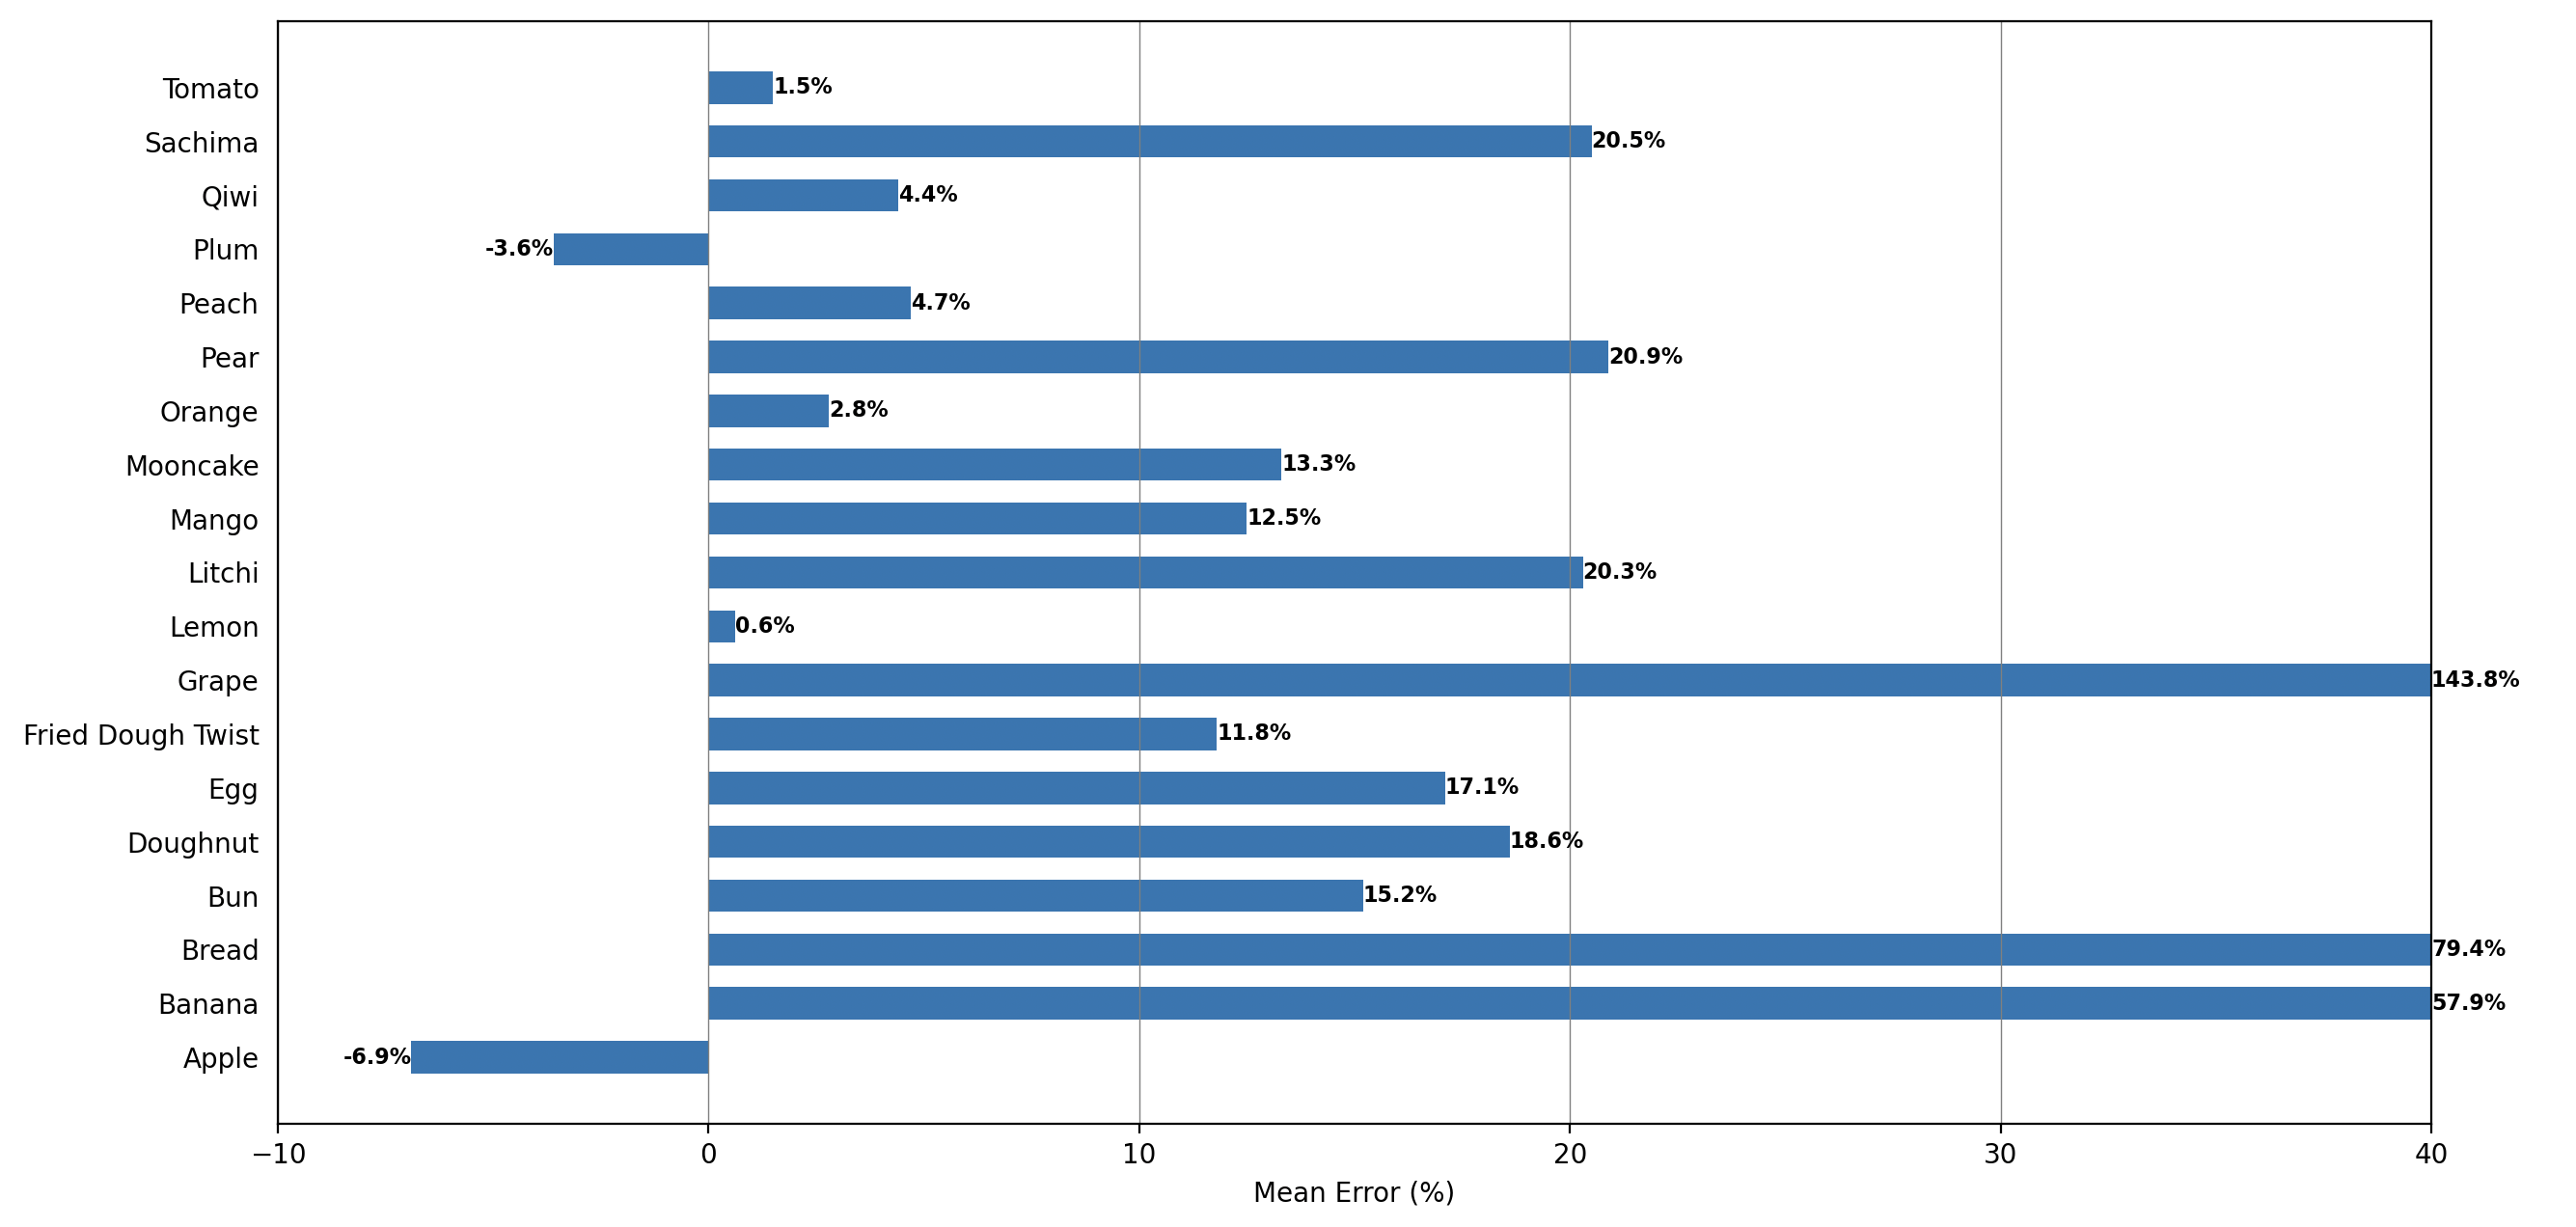
\includegraphics[width=\textwidth]{vol_est.png}
		\caption{\scriptsize Volume estimation results of food items from images}
	\end{figure}
	\begin{figure}[p]
		\centering
		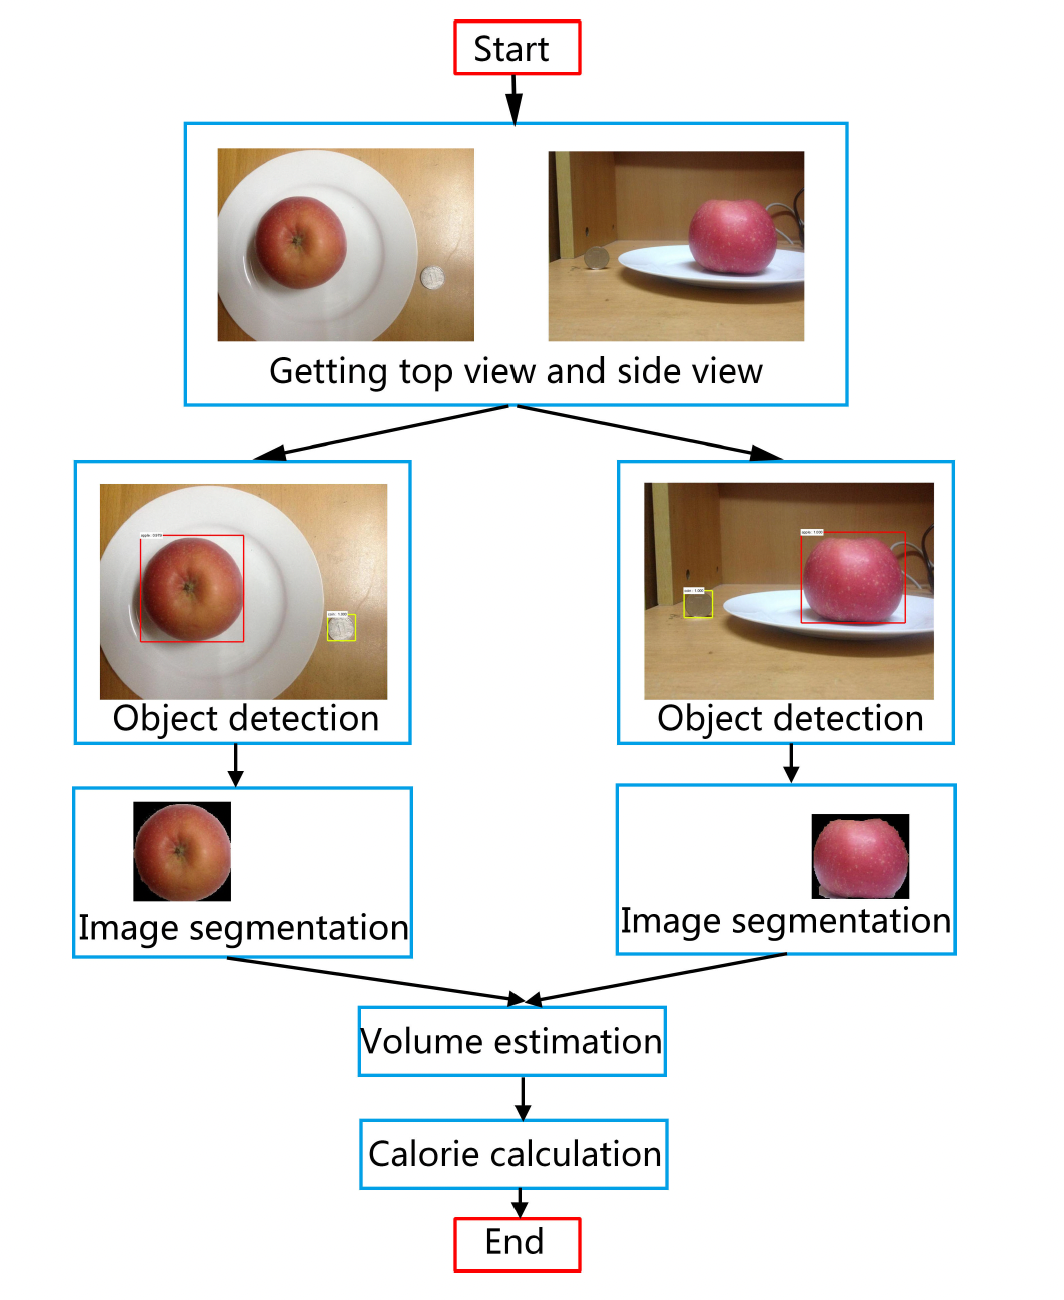
\includegraphics[width=\textwidth]{roadmap}
		\caption{Flowchart to implement the project\cite{liang}}
		\label{F:roadmap}
	\end{figure}
	
	\printbibliography
\end{document}